\documentclass[tikz,border=2mm]{standalone}

\usetikzlibrary{arrows,positioning}

\begin{document}

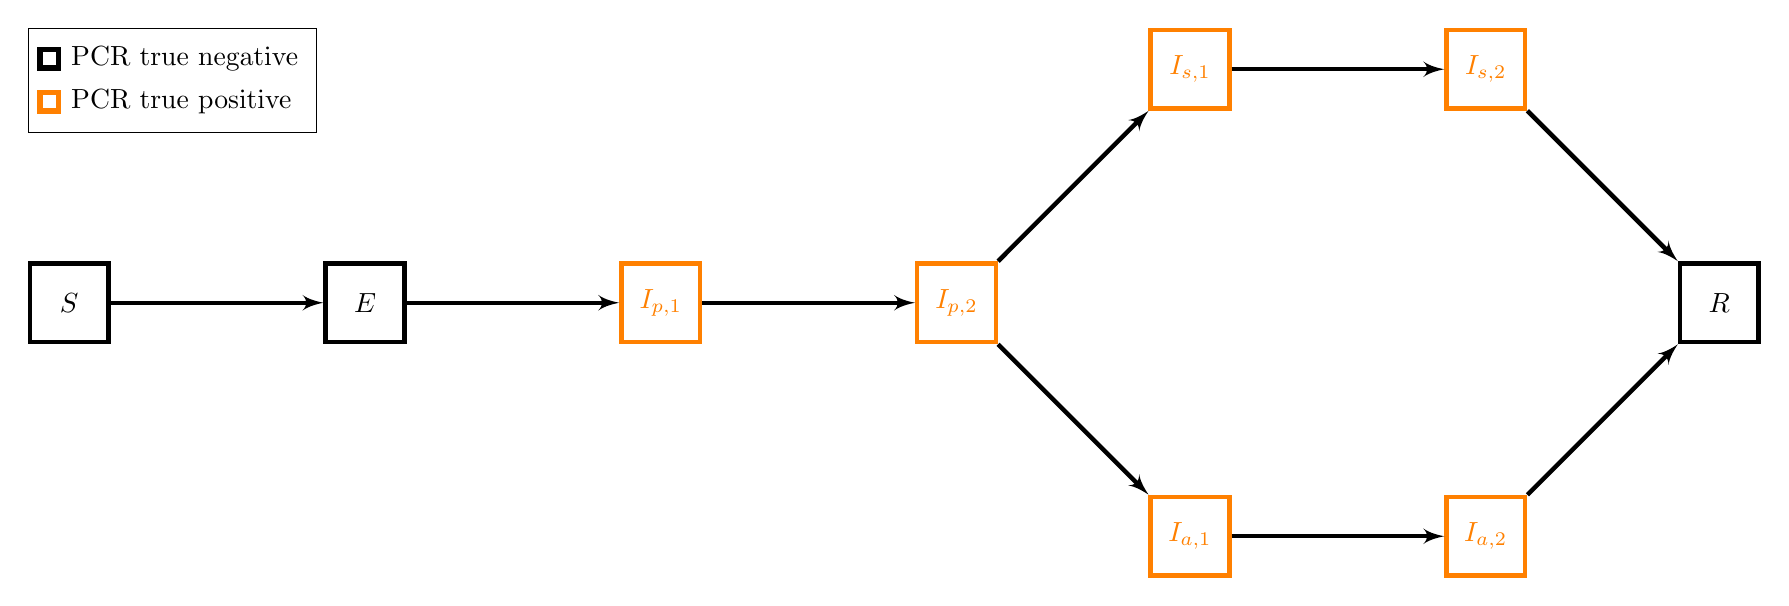
\begin{tikzpicture}[node distance=2.7cm,auto,>=latex',every node/.append style={align=center},int/.style={draw, minimum size=1cm},inverter/.style={rectangle,draw,inner sep=2pt,minimum size=6mm},posnode/.style={shape=rectangle, draw=orange, line width=2},
  negnode/.style={shape=rectangle, draw=black, line width=2}]
    \node [int, ultra thick] (S)             {$S$};
    \node [int, right=of S, ultra thick] (E)             {$E$};
    \node [int, right=of E, ultra thick, orange] (Ip1)             {$I_{p,1}$};
    \node [int, right=of Ip1, ultra thick, orange] (Ip2)             {$I_{p,2}$};
    \node [int, above right=of Ip2, ultra thick, orange] (Is1)             {$I_{s,1}$};
    \node [int, right=of Is1, ultra thick, orange] (Is2)             {$I_{s,2}$};
    \node [int, below right=of Ip2, ultra thick, orange] (Ia1)             {$I_{a,1}$};
    \node [int, right=of Ia1, ultra thick, orange] (Ia2)             {$I_{a,2}$};
    \node [int, below right=of Is2, ultra thick] (R)             {$R$};
    \path[->, ultra thick] (S) edge (E);
    \path[->, ultra thick] (E) edge (Ip1);
    \path[->, ultra thick] (Ip1) edge (Ip2);
    \path[->, ultra thick] (Ip2) edge (Is1);
    \path[->, ultra thick] (Is1) edge (Is2);
    \path[->, ultra thick] (Ip2) edge (Ia1);
    \path[->, ultra thick] (Ia1) edge (Ia2);
    \path[->, ultra thick] (Is2) edge (R);
    \path[->, ultra thick] (Ia2) edge (R);
    \matrix [draw,below right] at (current bounding box.north west) {
        \node [negnode,label=right:PCR true negative] {}; \\
        \node [posnode,label=right:PCR true positive] {}; \\
    };
\end{tikzpicture}
\end{document}